\section{Sensorik}
Für die Berechnung des Regelkreises müssen die Zustandsgrößen erfasst erfasst werden, deshalb beschäftigt sich der folgende Abschnitt mit der verwendeten Sensorik und derer Auswertung. Hierfür müssen die Sensoren in das mechanische Modell eingebunden werden um Messkennlinien zu bestimmen. Hierbei zeigt sich, dass mehrere Möglichkeiten bestehen die verschiedenen Größen zu ermitteln. Eine Vorarbeit hat gezeigt, dass diese von unterschiedlichen Störungen betroffen sind, weshalb Methoden erarbeitet werden müssen um einen qualitativen Vergleich zu ermöglichen. 

\begin{figure}[!h]
\centering
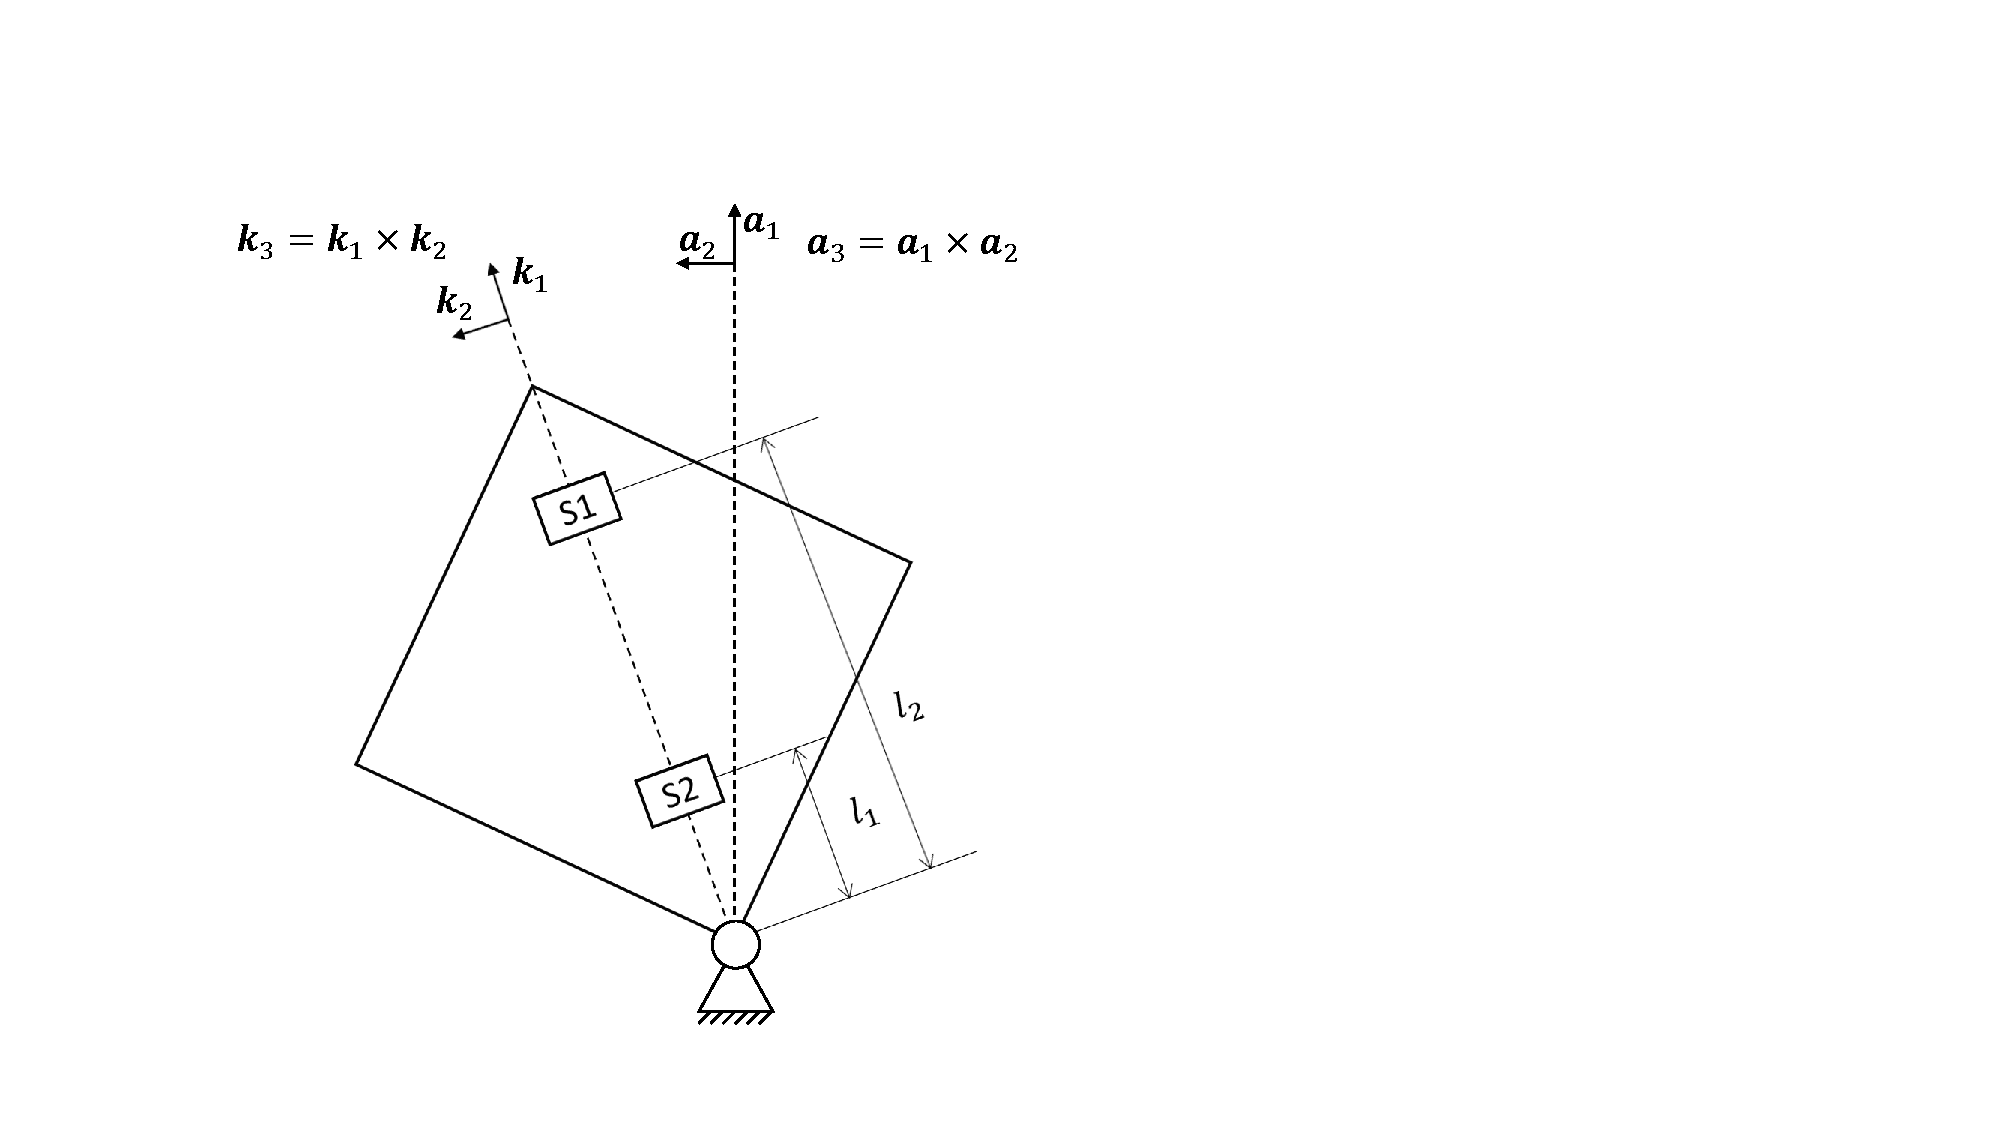
\includegraphics[width=0.6\linewidth, trim={1cm 1.5cm 18cm 3.5cm}, clip]{3_Sensorik/img/SensorAnordnung}
\caption{Anordnung der Sensoren an der Würfelseite, Quelle: eigene Darstellung}
\end{figure}

An der Würfelseite sind zwei MPU6050-ICs angebracht, um die Größen $\varphi$, $\dot{\varphi}$ und $\ddot{\varphi}$ zu messen. Die ICs verfügen über einen Beschleunigungs- und Drehratensensor, welche jeweils Messwerte in Richtung von drei Achsen liefern. Zuerst müssen Messkennlinien ermittelt werden. Das heißt die Messwerte der Sensoren werden mit Hilfe des mechanischen Modells in Zusammenhang mit den Messgrößen $\varphi$, $\dot{\varphi}$ und $\ddot{\varphi}$ gebracht. 

Die Messwerte der Drehratensensoren entsprechen der Winkelgeschwindigkeit der Würfelseite im körperfesten Bezugssystem $K$.

\begin{equation}
\bs{\omega}_{S_i} = \begin{pmatrix}
\omega^{S_i}_x \\ \omega^{S_i}_y \\ \omega^{S_i}_z
\end{pmatrix} = \presuper{K}{\big(\vel{A}{\omega}{K}\big)} = \begin{pmatrix}
{0} \\ {0} \\ {\dot{\varphi}}
\end{pmatrix}
\end{equation}

Somit sind nur die Komponenten in Richtung der Z-Achse von Bedeutung. Diese werden als Messwerte $y_i$ definiert.

\begin{equation}
y_i \equiv \omega^{S_i}_z \hspace{35pt} y_i = \dot{\varphi} \hspace{35pt} (i=1, 2)
\end{equation}

Die Ausgabewerte $\bs{a}_{S_i}$ der Beschleunigungssensoren setzt sich, nach dem idealisierten Modell, aus zwei Termen zusammen. Der erste Term entspricht der Beschleunigung der Sensoren im raumfesten Bezugssystem $A$, welche gleich der zweiten Ableitung des Ortvektors $\bs{s}_i$ der Sensoren mit Respekt zu $A$ ist.

\begin{equation}
\begin{split}
\vel{A}{a}{S_i} &= \frac{\presuper{A}{d} \vel{A}{v}{S_i}}{dt} = \frac{\presuper{A}{d}}{dt}\big(\vel{A}{\bs{\omega}}{K} \times \bs{s}_i\big) = \frac{\presuper{A}{d}\vel{A}{\omega}{K}}{dt}\times \bs{s}_i + \vel{K}{\omega}{S_i} \times \frac{\presuper{A}{d}\bs{s}_i}{dt} \\
&= \vel{K}{\alpha}{S_i} \times \bs{s}_i + \vel{A}{\omega}{K} \times \big(\vel{A}{\omega}{K} \times \bs{s}_i\big)
\\
&= \vecBS{K}{0}{0}{\ddot{\varphi}} \times \vecBS{K}{l_i}{0}{0}  + \vecBS{K}{0}{0}{\dot{\varphi}} \times \begin{pmatrix}
\vecBS{K}{0}{0}{\dot{\varphi}} \times \vecBS{K}{l_i}{0}{0} 
\end{pmatrix} = \vecBS{K}{-\dot{\varphi}^2 \cdot l_i}{\ddot{\varphi}\cdot l_i}{0}
\end{split}
\end{equation}

Der zweite Term wird von der Gravitation beeinflusst. Das heißt er entspricht der Darstellung des Erdbeschleunigungsvektors im körperfesten Bezugssystem $K$.

\begin{equation}
\bs{g} = \pMat{A}{K} \cdot \vecBS{A}{-g}{0}{0} = \vecBS{K}{-g \cdot c_{\varphi}}{g \cdot s_{\varphi}}{0}
\end{equation}

Somit ergeben sich die folgenden Zusammenhänge für die Anzeigewerte $\bs{a}_{S_i}$ der Beschleunigungssensoren, welche wiederum als Messwerte $y_3,...,y_6$ definiert werden.

\begin{equation}
\bs{a}_{S_i} = \begin{pmatrix}
\ddot{x}_{S_i} \\ \ddot{y}_{S_i} \\ \ddot{z}_{S_i}
\end{pmatrix} = 
\presuper{K}{\big(\vel{A}{a}{S_i} + \bs{g}\big)} = \vecBS{K}{-\dot{\varphi}^2 \cdot l_i - g\cdot c_{\varphi}}{\ddot{\varphi}\cdot l_i + g \cdot s_{\varphi}}{0}
\end{equation}
\begin{equation}
\begin{split}
&y_3 \equiv a^{S_1}_x \hspace{35pt} y_3 = -\dot{\varphi}^2 \cdot l_1 - g \cdot c_{\varphi} \\
&y_4 \equiv a^{S_2}_x \hspace{35pt} y_4 = -\dot{\varphi}^2  \cdot l_2 - g\cdot c_{\varphi} \\
&y_5 \equiv a^{S_1}_y \hspace{35pt} y_5 = \ddot{\varphi} \cdot l_1 + g\cdot s_{\varphi} \\
&y_6 \equiv a^{S_2}_y \hspace{35pt} y_6 = \ddot{\varphi} \cdot l_2 + g\cdot s_{\varphi}
\end{split}
\end{equation}

\subsection{Untersuchung der Messsysteme für  $\dot{\varphi}$}
Die Winkelgeschwindigkeit der Würfelseite kann mit Hilfe der beiden Drehratensensoren gemessen werden. Da zwei dieser Sensoren verwendet werden kann ein dritter Messwert definiert werden, welcher der Mittlung der beiden Sensorwerte entspricht.
\begin{equation}
\begin{split}
y_1 \equiv \omega^{S_1}_z & y_1 = \dot{\varphi} \\
y_2 \equiv \omega^{S_2}_z & y_2 = \dot{\varphi} \\
y_3 \equiv \frac{y_1+y_2}{2} & y_3 = \dot{\varphi}
\end{split}
\end{equation}
Die drei Messsysteme besitzen die selbe Kennlinie und somit identische Empfindlichkeit, weshalb diese nicht als Bewertungskriterium verwendet werden kann. Allerdings können die Messwerte in der Ruhelage über einen Zeitraum $T$ aufgenommen werden. In dieser Messreihe verschwindet der Wert der Messgröße $\dot{\varphi}=0$. Deshalb handelt es sich bei den gemessenen Werten um reine Rauschsignale, derer Effektivwerte bestimmt werden können. Diese sollen als erstes Bewertungskriterium verwendet werden.
Aus der Messreihe über $n=8096$ Werte bei einer Abtastfrequenz $f_a=50Hz$ ergeben sich die folgenden Effektivwerte.
\begin{equation}
\begin{split}
R^{Eff}_1 &= \sqrt{\frac{1}{n}\sum^n_{k=1}{y_1(k)}^2} = 0.0010 \\
R^{Eff}_2 &= \sqrt{\frac{1}{n}\sum^n_{k=1}{y_2(k)}^2} = 0.0010 \\
R^{Eff}_3 &= \sqrt{\frac{1}{n}\sum^n_{k=1}{y_3(k)}^2} = 0.0007
\end{split}
\end{equation}
Der Effektivwert des Rauschens wird durch die Mittelung der beiden Sensorwerte minimiert. Deshalb wird der Messwert $y_3$ zur Bestimmung von $\dot{\varphi}$ verwendet.

\subsection{Ermittlung von $\varphi$}
Zuerst sollen die Möglichkeiten zur Bestimmung von $\varphi$ näher untersucht werden. Die Kennlinien der Beschleunigungssensoren zeigen, dass die momentane Ausrichtung der Würfelseite deren Anzeigewerte beeinflusst. Allerdings hängen die Beschleunigungswerte von weiteren Messgrößen ab, weshalb ein einzelner Wert nicht ausreicht um den Winkel $\varphi$ zu berechnen. Allerdings kann durch die gewichtete Differenz zweier Beschleunigungswerte der Einfluss der Winkelgeschwindigkeit und -beschleunigung eliminiert werden.
\begin{equation}
\begin{split}
y_9 \equiv y_3 - \frac{l_1}{l_2}y_4 &y_9 = -g\cdot c_{\varphi}\cdot (1-\frac{l_1}{l_2}) \\
y_{10} \equiv y_5 - \frac{l_1}{l_2}y_6 &y_{10} = g\cdot s_{\varphi}\cdot(1-\frac{l_1}{l_2}) \\
y_{11}\equiv \frac{y_{10}}{y_{11}} &y_{11} = -tan(\varphi)
\end{split}
\end{equation}
Als erstes Beurteilungskriterium werden die Empfindlichkeiten der Messsysteme verwendet, welche sich durch die partielle Ableitung der Kennlinien nach der Messgröße ergeben.
\begin{equation}
\begin{split}
S_9(\varphi) &= \frac{\partial y_9}{\partial \varphi} = g\cdot s_{\varphi}\cdot (1 - \frac{l_1}{l_2}) \\
S_{10}(\varphi) &= \frac{\partial y_{10}}{\partial \varphi} = g \cdot c_{\varphi} \cdot (1- \frac{l_1}{l_2}) \\
S_{11}(\varphi) &= \frac{\partial y_{11}}{\partial \varphi} = -tan(\varphi)^2 - 1
\end{split}
\end{equation}
\begin{figure}[h!]
\centering
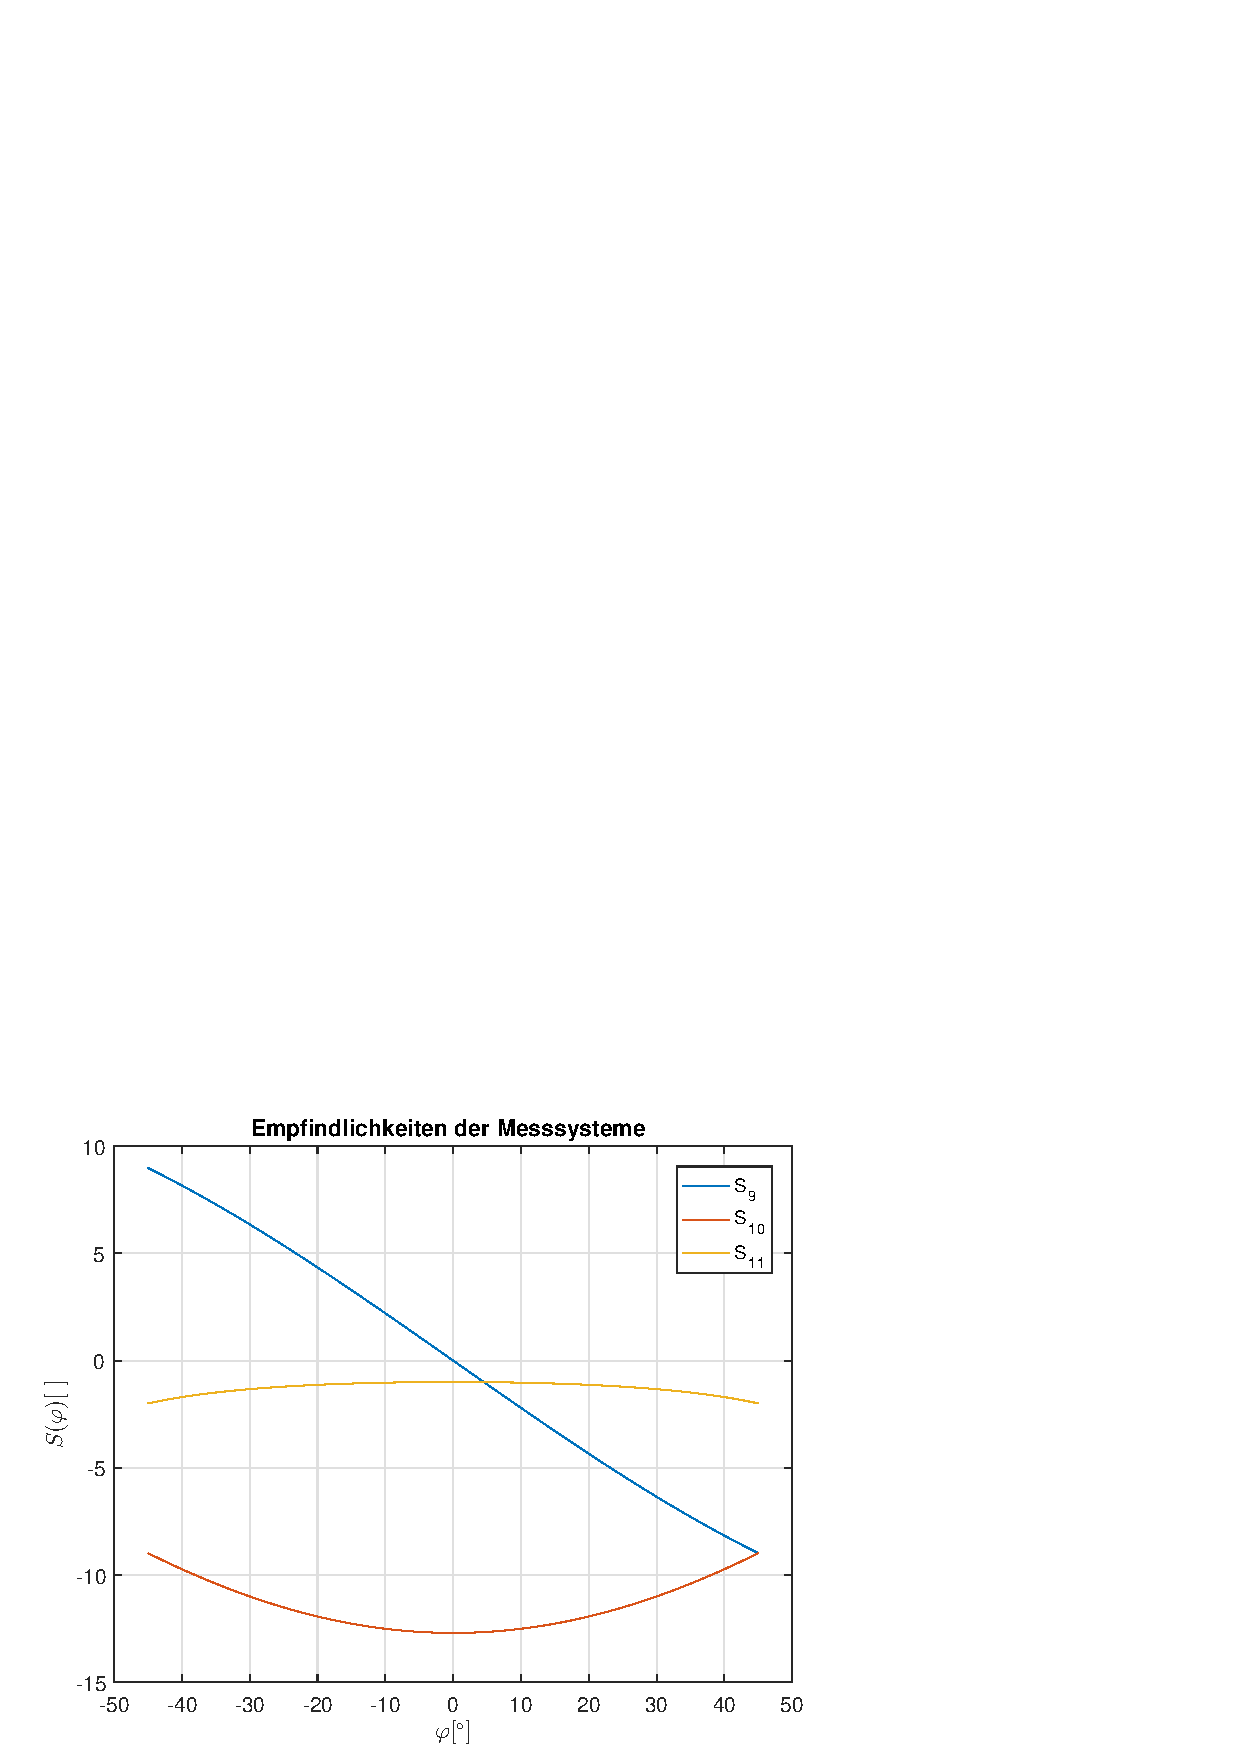
\includegraphics[width=0.5\linewidth]{3_Sensorik/img/empfindlichkeit_phi}
\caption{Empfindlichkeiten für $\varphi$, Quelle: eigene Darstellung}
\end{figure}
In der Abbildung ist deutlich zu erkennen, dass der Messwert $y_{10}$ die höchste Empfindlichkeit besitzt. Hieraus folgt, dass bereits kleine Änderung der Messgröße zu einer deutlichen Änderung des Messwertes führen. Folglich ist zu erwarten, dass das Signal-Rausch-Verhältnis mit zunehmender Empfindlichkeit größer wird.
Um die Signal-Rausch-Verhältnisse der Messsysteme zu bestimmen, wird die Würfelseite in einer bekannten Ausrichtung fixiert. Dadurch entsteht ein stationärer Prozess und es kann angenommen werden, dass der Mittelwert des Signales dem Nutzsignal entspricht. Die folgende Abbildung zeigt den Verlauf der Messgröße $\varphi$ aus den drei Messsystemen.

\begin{figure}[h!]
\centering
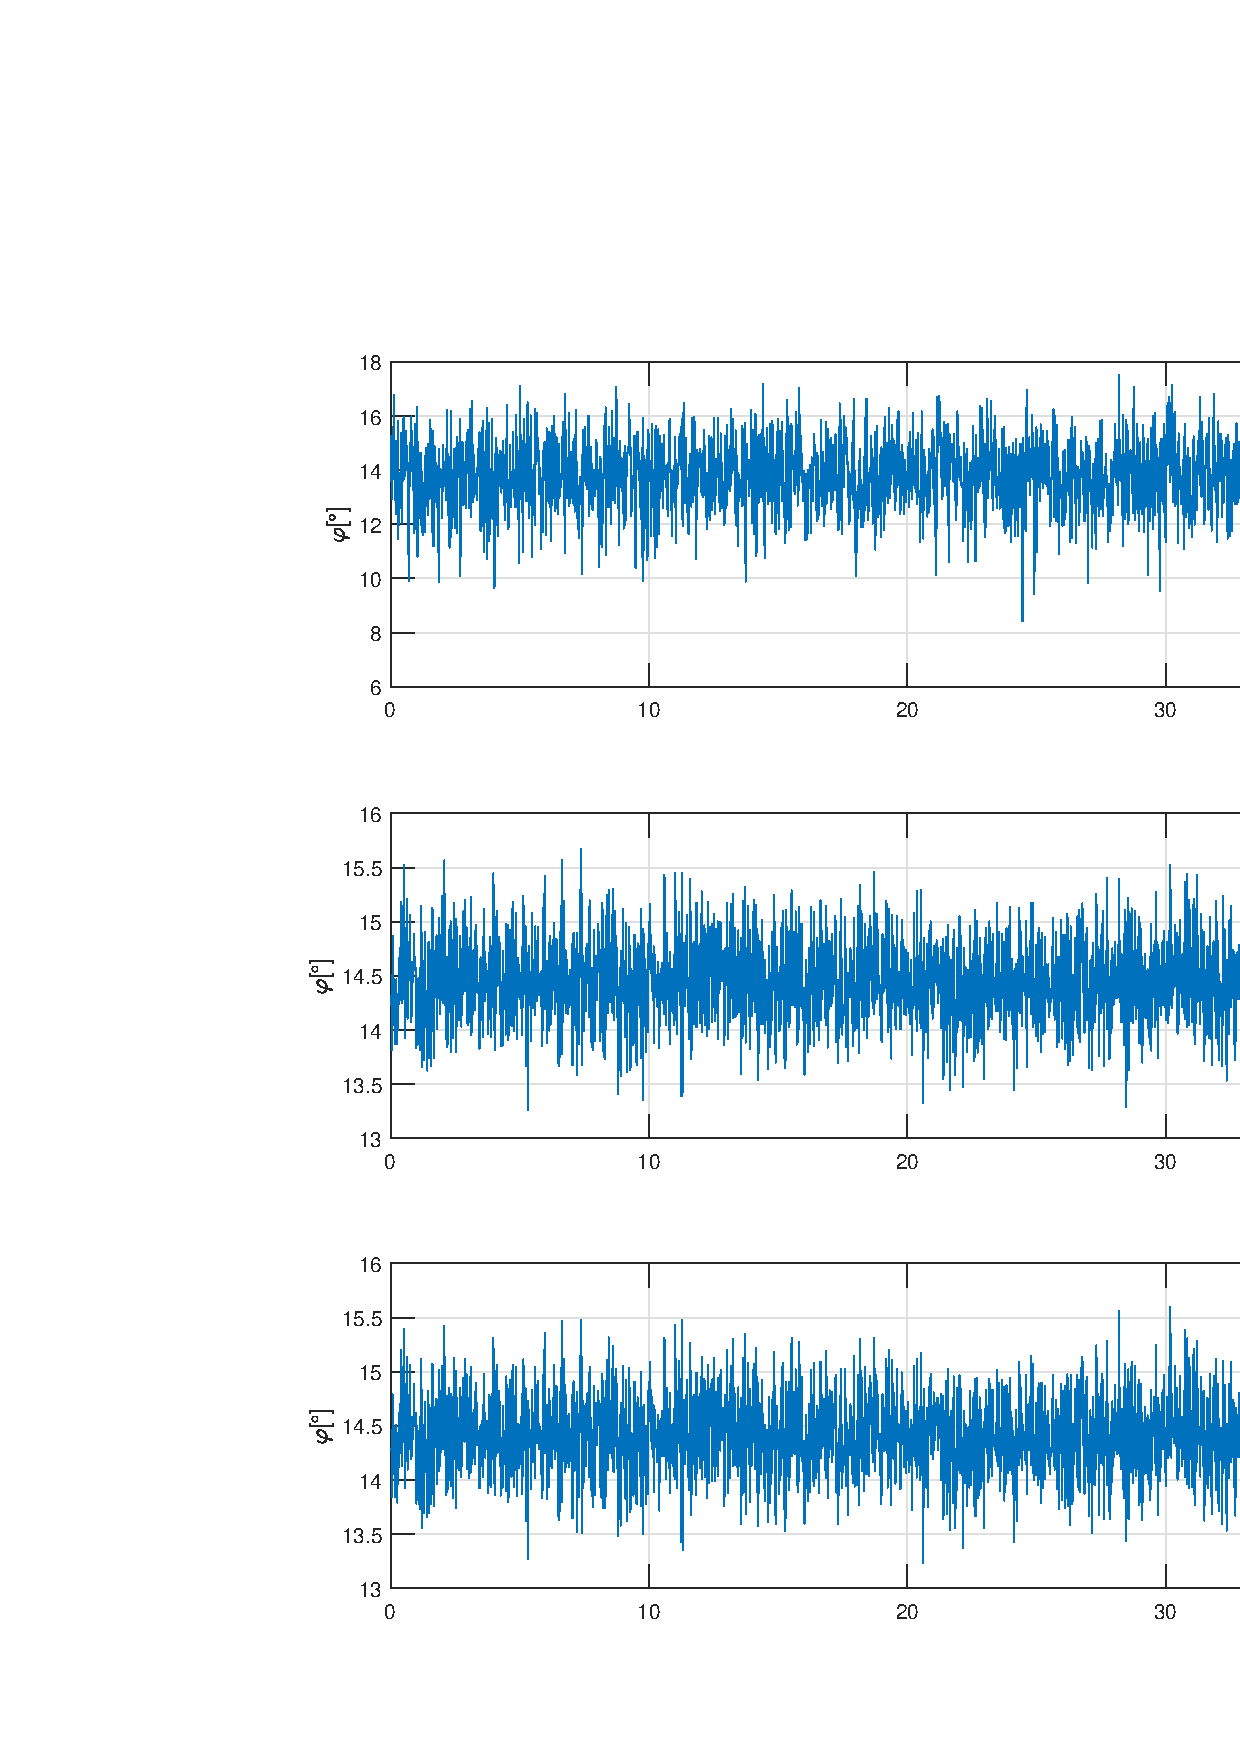
\includegraphics[width=\linewidth]{3_Sensorik/img/snr_phi_plot}
\caption{Signal-Rausch-Verhältnis der $\varphi$-Messsysteme, Quelle: eigene Darstellung}
\end{figure}

Die resultierenden Signal-Rausch-Verhältnisse sind:
\begin{equation}
SNR(y_9) = 20.57dB \hspace{35pt}  SNR(y_{10}) = 31.21dB \hspace{35pt} SNR(y_{11})=31.50dB
\end{equation}

Hier zeigt sich, dass das SNR von $y_{11}$ trotz niedriger Empfindlichkeit am höchsten ist. Einen mögliche Ursache hierfür ist, dass es sich bei dem Rauschen nicht um rein zufällige Signale handelt sondern diese von Störeinflüssen wie z.B. der Temperatur abhängen. Die Temperatur fließt nach Hersteller als weitere Proportionalität in die Kennlinie ein und wird somit durch die Division zweier mehrere Messwerte gekürzt. Weshalb die Division der beiden Messwerte zu einem verbesserten Signal-Rausch-Verhältnis führt.
In einer Vorarbeit hat sich herausgestellt, dass die Winkelschätzung aus den Beschleunigungssensoren bei hochfrequenten Anregungen von starken Störungen betroffen sind. Deshalb wird neben 
Neben den Beschleunigungssensoren kann der Winkel $\varphi$ auch aus den integrierten Winkelgeschwindigkeiten berechnet werden. Somit ergeben sich die beiden Schätzungen für den Winkel $\varphi$.
\begin{equation}
\varphi_A = -atan(y_{11}) \hspace{35pt} \varphi_G = \int y_3 dt
\end{equation}
Um die bereits angesprochen Störungen der Beschleunigungssensoren bei hochfrequenter Anregung zu untersuchen werden im nächsten Schritt Schwingversuche durchgeführt. Hierfür wird die Würfelseite als gewöhnliches Pendel aufgehängt, wodurch sich das Vorzeichen des Gravitationsmomentes ändert. Somit ergibt sich die folgende Zustandsraumdarstellung.

\begin{equation}
\dot{\bs{x}}=\bs{A}\cdot \bs{x}+\bs{B}\cdot \bs{u}
\end{equation}
\begin{equation}
\bs{A} = \begin{pmatrix}
 0 & 1 & 0 \\
 \frac{-m_G\cdot g\cdot l_C}{I^{K/O}+m_r\cdot l^2_M} & 
 \frac{-C_{\varphi}}{I^{K/O}+m_r\cdot l^2_M} &
 \frac{C_{\psi}}{I^{K/O}+m_r\cdot l^2_M} \\
 \frac{m_G\cdot g \cdot l_C}{I^{K/O}+m_r\cdot l^2_M} &
 \frac{C_{\varphi}}{I^{K/O}+m_r\cdot l^2_M} &
 \frac{C_{\psi}}{I^{G/O}(I^{K/O}+m_r\cdot l^2_M)}
\end{pmatrix}
\hspace{35pt}
\bs{B} = \begin{pmatrix}
0 \\ \frac{1}{I^{K/O}+m_r\cdot l^2_M} \\ \frac{I^{G/O}}{I^{R/M}(I^{K/O}+m_r \cdot l^2_M}
\end{pmatrix}
\end{equation}

\begin{equation}
\bs{y} = \begin{pmatrix}
\varphi
\end{pmatrix}
\end{equation}
\begin{equation}
\bs{y} = \bs{C} \cdot \bs{x} + \bs{D} \cdot \bs{u}
\end{equation}
\begin{equation}
\bs{C} = \begin{pmatrix}
1 & 0 & 0 
\end{pmatrix}
\hspace{35pt}
\bs{D} = \begin{pmatrix}
0
\end{pmatrix}
\end{equation}

Mit Hilfe der Zustandsraumdarstellung kann die Übertragungsfunktion $G(s)$ im Bildbereich berechnet werden.s